\documentclass[12pt, a4paper]{article}

\usepackage[utf8]{inputenc}
\usepackage[T1]{fontenc}
\usepackage{geometry}
\usepackage{hyperref}
\usepackage{amsmath}
\usepackage{amssymb}
\usepackage{booktabs}
\usepackage[backend=biber, style=authoryear]{biblatex}
\usepackage{tikz}
\usetikzlibrary{positioning}

\geometry{margin=2.5cm}
\addbibresource{references.bib}

\title{Image Fragment Reconstruction:\\
A Siamese Network Approach via Adjacency Prediction}
\author{}
\date{\today}

\begin{document}

\maketitle
\tableofcontents
\newpage

% ─────────────────────────────────────────────
\section{Problem Statement}
% ─────────────────────────────────────────────

Let $\mathcal{I} = \{I_1, \dots, I_N\}$ be a set of $N$ source images, each of spatial
resolution $H \times W \times 3$. Each image is divided into a regular $G \times G$ grid
of non-overlapping fragments of size $\frac{H}{G} \times \frac{W}{G} \times 3$, yielding
$G^2$ fragments per image and $M = N \cdot G^2$ fragments in total. In the experimental
setting used here $N = 10$, $H = W = 64$, $G = 4$, giving fragments of size
$16 \times 16 \times 3$ and $M = 160$ fragments per batch.

Let $f_k \in \mathbb{R}^{16 \times 16 \times 3}$ denote fragment $k$, and let
$s(k) \in \{1, \dots, N\}$ be its source image. The fragments from all $N$ images are
pooled into a single unordered collection. The task is:

\begin{quote}
\textit{Given the pooled collection of $M$ fragments with no positional or source
information, assign each fragment to one of $N$ groups such that all fragments assigned
to the same group originate from the same source image.}
\end{quote}

Formally, the goal is to recover a partition $\hat{\mathcal{C}} = \{\hat{C}_1, \dots,
\hat{C}_N\}$ of $\{1, \dots, M\}$ such that for each predicted cluster $\hat{C}_n$ there
exists a source image $I_{s}$ with $s(k) = s$ for all $k \in \hat{C}_n$.

\paragraph{Constraints.}
Two constraints make this non-trivial:

\begin{enumerate}
    \item \textbf{No positional information.} The original grid coordinates of each
          fragment are not provided at inference time. The model may not use absolute
          position as a feature.
    \item \textbf{No labels during training.} The source identity $s(k)$ is never
          provided to the model as a supervisory signal. The model must learn from
          structural properties of the fragments themselves.
\end{enumerate}

\paragraph{Known structure.}
Although labels are withheld, the following quantities are known and may be exploited:
\begin{itemize}
    \item The total number of source images $N = 10$ (so $k = N$ clusters are sought).
    \item Each source image contributes exactly $G^2 = 16$ fragments, so all clusters
          have equal size.
    \item Spatial adjacency within a source image is fully determined by the grid
          structure and can be derived without labels: fragments at grid positions
          $(r, c)$ and $(r', c')$ are adjacent if and only if $|r - r'| + |c - c'| = 1$.
\end{itemize}

The third point is the key observation exploited by the proposed approach (Section~2).

% ─────────────────────────────────────────────
\section{Related Work}
% ─────────────────────────────────────────────

The problem sits at the intersection of self-supervised representation learning and
clustering. We review three families of prior work that informed the approach.

\paragraph{Pretext-task self-supervision.}
The dominant paradigm in self-supervised vision until the rise of contrastive methods
was to define a hand-crafted pretext task whose labels are derivable from the data
itself. \textcite{noroozi2016} solve a jigsaw permutation: given a $3 \times 3$ grid
of fragments shuffled by one of 100 fixed permutations, predict which permutation was
used. The encoder learns features useful for downstream classification. Our adjacency
prediction is a much simpler, binary variant of this idea --- rather than predicting
a discrete permutation index over an exponentially large space, we predict a binary
label per pair. This trades off representational richness for sample efficiency.

\paragraph{Contrastive learning.}
SimCLR \parencite{simclr2020} and MoCo \parencite{moco2020} learn representations by
pulling together augmented views of the same image and pushing apart views of
different images. In the present setting these methods are awkward: there is no
natural positive pair construction, since the natural ``view'' of a fragment is the
fragment itself. One could treat all fragments from one source image as positives
of each other, but this requires the source label that we are explicitly forbidden
to use during training. Adjacency labels, in contrast, are derivable from the grid
structure alone.

\paragraph{Clustering-based self-supervision.}
DeepCluster \parencite{deepcluster2018} alternates between clustering current
embeddings and using cluster assignments as pseudo-labels. SwAV
\parencite{swav2020} extends this with online clustering and equipartitioned cluster
assignments via the Sinkhorn algorithm. Both are conceptually well-suited to this
task, but they introduce significant complexity (alternating training, prototype
maintenance) for what is at heart a small-scale clustering problem with $N = 10$
images. We treat this family as a strong candidate for follow-up work but defer it.

% ─────────────────────────────────────────────
\section{Core Idea}
% ─────────────────────────────────────────────

The central observation is that two fragments cut from the same image and placed next to
each other in the grid share a common boundary — colours bleed over, textures continue,
and objects span tiles. This visual continuity is a strong and reliable signal that does
not require any human annotation to exploit: since the experimenter creates the grid, the
ground-truth adjacency of every fragment pair is known at all times.

The proposed approach uses adjacency prediction as a \textbf{pretext task}
\parencite{noroozi2016}. The model is trained to solve a surrogate problem — predicting
whether two fragments are spatially adjacent — and in doing so is forced to learn visual
representations that capture source identity as a side effect. At inference time the
pretext objective is discarded and the learned representations are used for clustering.

This is self-supervised throughout: no labels beyond those derivable from the grid
structure are ever used.

% ─────────────────────────────────────────────
\section{Why Adjacency Prediction Helps}
% ─────────────────────────────────────────────

The naive contrastive approach (Section 3 of the companion document) faces a fundamental
tension: intra-image fragments can be visually dissimilar (a sky tile vs.\ a ground tile
from the same photograph), while inter-image fragments can be visually similar (two sky
tiles from different photographs). Adjacency prediction addresses this directly:

\begin{itemize}
    \item To predict whether two fragments are adjacent, the model must first determine
          whether they could plausibly come from the same image at all — source identity
          is a necessary precondition for adjacency.
    \item Adjacency exploits \textbf{local edge continuity} — a signal that is
          orthogonal to global visual similarity and therefore less susceptible to the
          sky-tile problem.
    \item The pretext task is harder than simple contrastive learning, which forces the
          model to learn richer representations.
\end{itemize}

% ─────────────────────────────────────────────
\section{Architecture: Siamese Network}
% ─────────────────────────────────────────────

The model consists of two components:

\paragraph{Shared CNN encoder.}
A single convolutional neural network maps each 16$\times$16$\times$3 fragment to a
256-dimensional embedding vector. The architecture is three convolutional blocks
(Conv--BatchNorm--ReLU), with max-pooling after blocks two and three, reducing the
spatial dimensions from $16\times16$ to $4\times4$. The flattened $4\times4\times128$
feature map is projected to a 256-dimensional embedding via a linear layer followed by
ReLU and dropout ($p=0.3$).

The encoder is \textbf{shared} — the same weights are used for both fragments in a pair.
This is the defining property of a Siamese network \parencite{siamese1994}: weight
sharing ensures that the comparison is symmetric and that the encoder learns a universal
fragment representation rather than one tuned to a specific input slot.

\paragraph{Comparison head (MLP).}
A small multi-layer perceptron takes as input a 1024-dimensional vector formed by
concatenating four interaction terms between the two embeddings $\mathbf{a} =
\text{CNN}(f_i)$ and $\mathbf{b} = \text{CNN}(f_j)$:

\[
\mathbf{z}_{ij} = \bigl[\mathbf{a} - \mathbf{b} \;\|\; \mathbf{a} \odot \mathbf{b} \;\|\; \mathbf{a} \;\|\; \mathbf{b}\bigr] \in \mathbb{R}^{1024}
\]

The difference $\mathbf{a} - \mathbf{b}$ captures asymmetric discrepancies; the
element-wise product $\mathbf{a} \odot \mathbf{b}$ captures feature co-activation; and
including both raw embeddings preserves their individual information. The MLP maps
$\mathbf{z}_{ij}$ through a hidden layer of size 128 (ReLU) to a single scalar in
$[0, 1]$:

\[
p_{ij} = \sigma\!\bigl(W_2\,\text{ReLU}(W_1\,\mathbf{z}_{ij} + b_1) + b_2\bigr)
\]

% ─────────────────────────────────────────────
\section{Training}
% ─────────────────────────────────────────────

\subsection{Constructing Training Labels}

From a sample of 10 images cut into a 4$\times$4 grid, each fragment has at most 4
adjacent neighbours (fewer at corners and edges). For a sample of 160 fragments the
total number of pairs is:

\[
\binom{160}{2} = 12{,}720
\]

Each pair receives a binary label: $y_{ij} = 1$ if the two fragments are adjacent within
the same image, $y_{ij} = 0$ otherwise. This label is derived entirely from the known
grid positions and requires no human annotation.

\subsection{Class Imbalance}

Adjacent pairs are rare relative to non-adjacent pairs. Within one image of 16 fragments
there are 24 adjacent pairs and $\binom{16}{2} - 24 = 96$ non-adjacent same-image pairs,
plus all cross-image pairs. Across the full 160-fragment sample the positive rate is low.
This imbalance should be addressed via weighted loss or by subsampling negatives during
training.

\subsection{Loss Function}

Binary cross-entropy is the natural loss for a binary prediction task:

\[
\mathcal{L}_{\text{BCE}} = -\frac{1}{N}\sum_{(i,j)} \Bigl[ y_{ij} \log p_{ij} + (1 - y_{ij}) \log(1 - p_{ij}) \Bigr]
\]

Positive (adjacent) pairs are far rarer than negative pairs in this configuration.
With 10 source images on a $4 \times 4$ grid, each image contributes
$4 \cdot 3 + 3 \cdot 4 = 24$ adjacent pairs, giving $n_{+} = 240$ positives in
total. The remaining pairs are negatives: $n_{-} = \binom{160}{2} - 240 = 12{,}480$.
The ratio $n_{-}/n_{+} = 52$ is therefore a constant determined by the grid
geometry, not a per-batch quantity. Vanilla BCE on this data is dominated by the
negative class: the gradient is overwhelmingly driven by the loss on non-adjacent
pairs, and the model has little incentive to identify the few adjacent ones. The
standard remedy is to upweight the rare class. Since only the ratio of the two
class weights matters, we parameterise the loss with a single \emph{tilt}
parameter $\beta \geq 1$:
\[
\mathcal{L}_{\text{WBCE}}(\beta) = -\frac{1}{N}\sum_{(i,j)}
    \Bigl[\, \beta \cdot \tfrac{n_{-}}{n_{+}}\, y_{ij} \log p_{ij}
       + (1 - y_{ij}) \log(1 - p_{ij}) \,\Bigr].
\]

The textbook value is $\beta = 1$, the class-balanced loss: it equalises the
total gradient contribution of the two classes, treating a single positive as
worth 52 negatives. Setting $\beta > 1$ over-weights positives beyond this
point --- a positive mistake is now \emph{more} costly than the natural class
ratio implies. For our downstream task this is desirable, and we expect the
optimum to lie at a moderate-to-aggressive tilt.

\paragraph{Why we lean toward a moderate-to-aggressive tilt.}
The downstream task is graph clustering, not per-edge classification. False
negatives directly weaken intra-cluster connectivity, while false positives are
only harmful when they connect fragments from \emph{different} source images ---
a case the model rarely produces because cross-image fragments are visually
dissimilar. Same-image false positives, the more common kind, actually reinforce
the connectivity spectral clustering relies on. The error costs are therefore
asymmetric in favour of recall, and we expect the optimal $\beta$ to lie above
the class-balanced point.

\subsection{Computational Cost}

The CNN encoder runs once per fragment (160 forward passes per sample). All pairwise
embeddings are then combined using tensor operations, and the lightweight MLP processes
all 12,720 pairs. Since the expensive step (the CNN) runs only 160 times, the
computational overhead is manageable.

% ─────────────────────────────────────────────
\section{From Pretext Task to Clustering}
% ─────────────────────────────────────────────

After training, the model produces a predicted probability $p_{ij}$ for every pair of
fragments. These probabilities define a \textbf{fully connected weighted graph} over the
160 fragments, where edge weight $w_{ij} = p_{ij}$ reflects the model's confidence that
fragments $i$ and $j$ are adjacent — and by extension, that they originate from the same
image (Figure~\ref{fig:similarity-graph}).

\begin{figure}[h]
\centering
% Standalone TikZ figure: predicted similarity graph over fragments.
%
% This file contains only the \begin{tikzpicture} ... \end{tikzpicture} block,
% so it can be \input{} into any host document that loads tikz. To preview as
% a standalone PDF, compile fig_similarity_graph_standalone.tex.

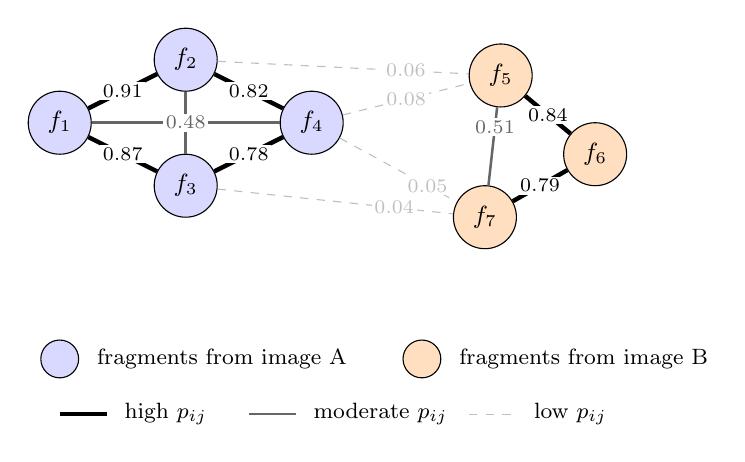
\begin{tikzpicture}[
    node/.style    = {circle, draw, minimum size=8mm, inner sep=0pt, font=\small},
    src1/.style    = {node, fill=blue!15},
    src2/.style    = {node, fill=orange!25},
    edge/.style    = {-, line width=0.6pt},
    strong/.style  = {edge, color=black, line width=1.6pt},
    medium/.style  = {edge, color=black!60, line width=0.9pt},
    weak/.style    = {edge, color=black!25, line width=0.4pt, dashed},
    weight/.style  = {font=\scriptsize, fill=white, inner sep=1pt},
]

% --- nodes: 4 fragments from image A (blue), 3 from image B (orange) ---
\node[src1] (a1) at (0, 2)         {$f_1$};
\node[src1] (a2) at (1.6, 2.8)     {$f_2$};
\node[src1] (a3) at (1.6, 1.2)     {$f_3$};
\node[src1] (a4) at (3.2, 2)       {$f_4$};

\node[src2] (b1) at (5.6, 2.6)     {$f_5$};
\node[src2] (b2) at (6.8, 1.6)     {$f_6$};
\node[src2] (b3) at (5.4, 0.8)     {$f_7$};

% --- intra-A edges (high probability, drawn strong) ---
\draw[strong] (a1) -- (a2) node[weight, midway] {$0.91$};
\draw[strong] (a1) -- (a3) node[weight, midway] {$0.87$};
\draw[strong] (a2) -- (a4) node[weight, midway] {$0.82$};
\draw[strong] (a3) -- (a4) node[weight, midway] {$0.78$};
\draw[medium] (a1) -- (a4) node[weight, midway] {$0.55$};
\draw[medium] (a2) -- (a3) node[weight, midway] {$0.48$};

% --- intra-B edges ---
\draw[strong] (b1) -- (b2) node[weight, midway] {$0.84$};
\draw[strong] (b2) -- (b3) node[weight, midway] {$0.79$};
\draw[medium] (b1) -- (b3) node[weight, near start] {$0.51$};

% --- cross edges (low probability, weak/dashed) ---
\draw[weak] (a4) -- (b1) node[weight, midway] {$0.08$};
\draw[weak] (a4) -- (b3) node[weight, near end] {$0.05$};
\draw[weak] (a2) -- (b1) node[weight, near end] {$0.06$};
\draw[weak] (a3) -- (b3) node[weight, near end] {$0.04$};

% --- legend ---
\begin{scope}[shift={(0, -1.0)}]
    \node[src1, scale=0.6] (lg1) at (0, 0) {};
    \node[anchor=west, font=\footnotesize] at (0.35, 0) {fragments from image A};

    \node[src2, scale=0.6] (lg2) at (4.6, 0) {};
    \node[anchor=west, font=\footnotesize] at (4.95, 0) {fragments from image B};
\end{scope}

\begin{scope}[shift={(0, -1.7)}]
    \draw[strong] (0, 0) -- (0.6, 0);
    \node[anchor=west, font=\footnotesize] at (0.7, 0) {high $p_{ij}$};

    \draw[medium] (2.4, 0) -- (3.0, 0);
    \node[anchor=west, font=\footnotesize] at (3.1, 0) {moderate $p_{ij}$};

    \draw[weak] (5.2, 0) -- (5.8, 0);
    \node[anchor=west, font=\footnotesize] at (5.9, 0) {low $p_{ij}$};
\end{scope}

\end{tikzpicture}

\caption{Schematic of the predicted similarity graph. Each node is a fragment; edge
weight $p_{ij}$ is the model's predicted adjacency probability. Edges within a true
source image (here, two illustrative source images shown in blue and orange) tend to
have high probability; cross-image edges have low probability. Spectral clustering
recovers the source-image partition by finding the cut that separates the
densely-connected sub-graphs.}
\label{fig:similarity-graph}
\end{figure}

\paragraph{Decision point: clustering on the graph.}
\textbf{Spectral clustering} is the natural choice for a weighted graph. It uses the
eigenstructure of the graph Laplacian to find clusters that are internally
well-connected and externally weakly connected. With $k = 10$ known clusters, the
$k$ smallest eigenvectors of the Laplacian are used.

This is more principled than applying $k$-means directly to embeddings, because the
graph structure captures the full relational information between all fragment pairs
rather than just the position of individual embeddings in space.

\paragraph{Balanced spectral clustering.}
The standard spectral algorithm ignores the fact that each true cluster contains
exactly $G^2 = 16$ fragments, and can produce clusters of very unequal sizes. We
enforce balance by computing the $k$-dimensional spectral embedding (leading
eigenvectors of the normalised Laplacian via \texttt{sklearn.manifold.SpectralEmbedding})
and then assigning fragments to clusters with a Hungarian algorithm: each cluster is
expanded into $G^2$ slots, giving a $160 \times 160$ cost matrix on which
\texttt{scipy.optimize.linear\_sum\_assignment} returns a one-to-one assignment that
respects the per-cluster capacity. Centroids are then re-estimated and the assignment
is iterated until convergence (typically a handful of iterations).

\paragraph{Metric consistency.}
Unlike the contrastive approach, there is no distance metric to align between training
and clustering — the edge weights are probabilities produced directly by the model, and
spectral clustering operates on those weights natively.

% ─────────────────────────────────────────────
\section{Evaluation Metric: Adjusted Rand Index}

The primary evaluation metric is the \textbf{Adjusted Rand Index (ARI)}. It measures
how well the predicted clusters match the true groupings by counting fragment pairs:

\begin{itemize}
    \item A pair is a \textbf{true positive} if both fragments are in the same true group
          and the same predicted cluster.
    \item A pair is a \textbf{true negative} if they are in different true groups and
          different predicted clusters.
    \item All other pairs are errors.
\end{itemize}

The ``adjusted'' part corrects for chance — a random clustering would score
$\text{ARI} = 0$, a perfect clustering scores $\text{ARI} = 1$, and a clustering
worse than random can score below zero.

ARI is preferred over simpler metrics such as purity because purity only looks at the
dominant class in each cluster and ignores how errors are distributed. For example, a
cluster containing 60\% of fragments from image A and 40\% from image B scores the same
purity as a cluster containing 60\% from image A, 20\% from image B, and 20\% from image
C — despite the latter being more disordered. ARI captures this distinction.

\textbf{NMI (Normalised Mutual Information)} is reported alongside ARI as a
complementary metric. It measures how much information the predicted clusters share with
the true groupings, normalised to $[0, 1]$.

\paragraph{Multi-batch averaging.}
Each evaluation step samples a fresh batch of 10 source images from the validation
generator. Because individual batches vary substantially in difficulty (some draws of
10 ImageNet classes are visually well-separated, others contain near-duplicates), a
single-batch ARI estimate has high variance. We average each metric over
$n_{\text{eval}} = 20$ fresh validation batches per evaluation step. This stabilises
the training curves and, crucially, the early-stopping decision and the
checkpoint-selection criterion, which would otherwise be biased toward lucky batches.

% ─────────────────────────────────────────────
\section{Experimental Setup}
% ─────────────────────────────────────────────

\paragraph{Data.}
ImageNet-64 \parencite{imagenet64}: a downsampled version of the ImageNet-1k
classification dataset in which every image has been resized to $64 \times 64$
pixels. The dataset is split into a training partition and a test partition; we draw
the model's training images from the former and the validation images from the
latter. Each training step samples 10 random images on the fly and produces a fresh
batch of 160 fragments; the data generator is therefore effectively infinite. The
augmentation pipeline (rotation up to $\pm 20^\circ$, horizontal/vertical shift up
to 10\%, channel shift 0.2) is applied to the full image \emph{before} fragmentation
and is provided by the dataset's data generator (\texttt{data.py}); it is not
modified.

\paragraph{Hardware.}
All training and evaluation reported in this document was performed on a MacBook Air
(Apple M-series CPU). PyTorch is configured to fall back to CPU; no GPU is required.
A full training run completes in approximately 20--25 minutes on this hardware.

\paragraph{Reproducibility.}
\begin{itemize}
    \item Each run writes its full configuration, training log, and best checkpoint
          into \texttt{runs/\{run\_name\}/}, and appends a one-line summary to
          \texttt{results.jsonl}. The configuration is therefore self-contained and
          re-runnable.
    \item Random seeds are fixed for the clustering routines
          (\texttt{random\_state = 42} in \texttt{sklearn.cluster.SpectralClustering},
          \texttt{KMeans}, and \texttt{SpectralEmbedding}). The PyTorch random seed is
          \emph{not} currently fixed, so model initialisation and the order of training
          batches vary between runs; this is by design --- repeated runs with different
          seeds give a sense of the variance in final ARI.
    \item Hyperparameters and run metadata are versioned in \texttt{config.yaml}.
\end{itemize}

\paragraph{Hyperparameters.}
The complete list of hyperparameters is maintained in \texttt{config.yaml} and may
still change in the course of further ablations. The current values are documented
there; this section will be replaced with a final hyperparameter table once the
study is complete.

% ─────────────────────────────────────────────
\section{Results}
% ─────────────────────────────────────────────

\subsection{Effect of the loss tilt parameter $\beta$}

We evaluated three settings of the WBCE tilt parameter --- $\beta \in
\{0.019, 0.3, 1.0\}$, corresponding respectively to plain unweighted BCE
($\beta \cdot 52 = 1$), a mild upweighting of positives, and the textbook
class-balanced weighting ($w_{+} = 52$). All three runs use the same
architecture, balanced spectral clustering, and validation averaging over
$n_{\text{eval}} = 20$ fresh batches.

\begin{center}
\begin{tabular}{lccc}
\toprule
\textbf{Run} & \textbf{$\beta$} & \textbf{Best ARI} & \textbf{AUROC / AUPRC} \\
\midrule
\texttt{plain\_bce}     & $0.019$ & $0.535$ & $0.969 \,/\, 0.432$ \\
\texttt{wbce\_beta\_03} & $0.3$   & $0.523$ & $0.973 \,/\, 0.435$ \\
\texttt{wbce\_beta\_1}  & $1.0$   & $0.462$ & $0.969 \,/\, 0.405$ \\
\bottomrule
\end{tabular}
\end{center}

\paragraph{Discussion.}
The choice of $\beta$ has an essentially negligible effect on AUROC: across two
orders of magnitude in $\beta$, ranking quality on the adjacency task varies by
less than a percentage point ($0.969$--$0.973$). What changes with $\beta$ is
the model's \emph{calibration} --- its tendency to push probabilities high or
low overall --- not the order in which it ranks pairs. Because spectral
clustering operates on the raw probabilities as edge weights, both ranking and
calibration matter for ARI, which is why ARI varies a little more than
AUROC ($0.46$--$0.54$).

The variation we observe in ARI is, however, on the same order as the
run-to-run noise we estimated by repeating $\beta = 0.3$ and $\beta = 1$ with
different random seeds: between repeated runs of the same configuration the
ARI changed by up to $\sim 0.05$, comparable to the differences between
configurations. The cleanest reading of the data is that \emph{within the
range tested, $\beta$ is a second-order knob}. Plain BCE performs at least as
well as any weighted variant we tried.

This contradicts the prior expectation expressed earlier in the document
that an aggressive tilt $\beta \in [1.5, 3]$ would be optimal. The argument
about asymmetric error costs (false negatives breaking intra-cluster
connectivity more than false positives) is not wrong in principle, but the
model already learns a near-optimal ranking under plain BCE, so the loss
weighting has little remaining effect on the downstream task. We adopt
plain BCE for simplicity in subsequent experiments.

\subsection{Headline numbers}

\begin{center}
\begin{tabular}{lcc}
\toprule
                                          & \textbf{Best ARI}  & \textbf{AUROC} \\
\midrule
Run 1 (single-batch eval, unbalanced)     & $0.787$            & --             \\
Plain BCE (multi-batch eval, balanced)    & $0.535$            & $0.969$        \\
\bottomrule
\end{tabular}
\end{center}

The apparent regression from $0.787$ to $0.535$ is almost entirely the
multi-batch averaging unmasking the variance of single-batch evaluation:
the original number was a single lucky draw, while the new number is the
mean over twenty fresh validation batches.

\paragraph{Cross-run comparison.}
\emph{(Placeholder for the markdown table produced by \texttt{compare\_runs.py},
plus the overlay plot \texttt{runs\_comparison.png}.)}

% ─────────────────────────────────────────────
\section{Failure Modes}
% ─────────────────────────────────────────────

\emph{Placeholder section. To be filled with concrete examples of fragments the
model cannot distinguish (e.g.\ near-uniform sky tiles, blurred patches, fragments
with no informative texture) and an estimate of the empirical ceiling on ARI imposed
by these intrinsically ambiguous cases.}

% ─────────────────────────────────────────────
\section{Decision Points Summary}
% ─────────────────────────────────────────────

\begin{center}
\begin{tabular}{lll}
\toprule
\textbf{Decision} & \textbf{Choice} & \textbf{Alternatives} \\
\midrule
Training objective & Adjacency prediction (pretext task) & Contrastive loss \\
Architecture & Siamese CNN + MLP head & Single encoder \\
Embedding combination & Diff $+$ product $+$ both embeddings & Concatenation only \\
Loss function & Binary cross-entropy & Focal loss (for imbalance) \\
Class imbalance & Weighted loss or negative subsampling & None \\
Clustering algorithm & Balanced spectral clustering & Plain spectral, $k$-means \\
Number of clusters & $k = 10$ (known) & Discovered automatically \\
Cluster size & Enforced ($G^2 = 16$) via Hungarian & Free \\
Eval batches per step & 20 (averaged) & 1 (single batch) \\
Evaluation metric & ARI, NMI & Purity \\
\bottomrule
\end{tabular}
\end{center}

% ─────────────────────────────────────────────
\section{Limitations}
% ─────────────────────────────────────────────

\begin{itemize}
    \item Adjacency is a local signal — it says nothing directly about fragments that are
          far apart within the same image. The model must generalise from local adjacency
          to global source identity.
    \item The graph has 12,720 edges. For larger grids or larger samples this grows
          quadratically and may become a bottleneck.
    \item The pretext metric and the task metric are misaligned. We train binary
          adjacency (only $\sim$1.9\% positives) but evaluate clustering. The model can
          achieve a useful similarity matrix (ARI $\approx 0.78$) while only mediocre
          on adjacency F1 ($\approx 0.26$), because adjacency is a sufficient but not
          necessary condition for same-source identity.
\end{itemize}

% ─────────────────────────────────────────────
\section{Further Suggestions}
% ─────────────────────────────────────────────

\paragraph{Multi-task loss combining adjacency and same-image prediction.}
The current loss optimises only adjacency, which is sparse ($\sim$1.9\% positive pairs)
and only indirectly aligned with the clustering task. A natural extension is to train
two heads jointly:

\[
\mathcal{L} = \lambda_{\text{adj}} \cdot \text{BCE}_{\text{adjacency}}
            + \lambda_{\text{same}} \cdot \text{BCE}_{\text{same-image}}
\]

The same-image label $y^{\text{same}}_{ij} = \mathbb{1}[s(i) = s(j)]$ is also free
(known from the grid construction), denser ($\sim$10\% positives), and directly
matched to what the spectral clustering will use downstream. Adjacency provides the
finer-grained, harder-to-learn signal; same-image prediction provides the dense
task-aligned signal. Tuning $\lambda_{\text{adj}}$ and $\lambda_{\text{same}}$ would
let us trade off between the two.

\paragraph{Recall-tilted adjacency objective.}
At inference time, spectral clustering does not need precise per-edge probabilities —
it needs the overall connectivity structure of the graph to be correct. A few
false-positive edges between same-image fragments are tolerable; missed adjacent edges
weaken the connectivity within a true cluster. This argues for tilting the adjacency
loss toward recall, e.g.\ via a higher positive-class weight, focal loss with
$\alpha > 0.5$, or an asymmetric BCE in which false negatives are penalised more
heavily than false positives. The current weighted BCE already partially does this;
further increasing the positive weight is worth ablating.

% ─────────────────────────────────────────────
\section*{TODO}
% ─────────────────────────────────────────────

\begin{itemize}
    \item \textbf{Limit model capacity} — a small CNN has less capacity to memorise than
          a large one. Justify the chosen architecture size explicitly in the report.
    \item \textbf{Color-histogram baseline} — implement a non-learned baseline
          (per-fragment color histograms with chi-square or EMD distance, then
          spectral clustering on the affinity matrix). This anchors the learned
          model's ARI against a meaningful reference.
\end{itemize}

\paragraph{Already implemented.}
Dropout ($p = 0.3$ after the encoder's projection layer), weight decay
($\lambda = 10^{-4}$ in the Adam optimiser), balanced spectral clustering (Hungarian
assignment with $G^2 = 16$ slots per cluster), and multi-batch averaged evaluation
($n_{\text{eval}} = 20$) are all active in the current implementation.

\printbibliography

\end{document}
